
\subsection{katz-eig}\label{sec:opt:katzeig}

The strategies for optimizing algorithm parameters for different datasets, or parameter tuning, has focuses on keeping $\beta$ fixed and searching for $K$ which optimizes \textit{F-measure}. The analysis in \sectionref{sec:param:katzeig} shows that varying $\beta$ has a neglible effect on the algorithm's performance, so $\beta$ is fixed as $\beta = \frac{1}{\|A_{train}\|_2}$.

What follows is a description of the different optimization strategies evaluated:

\begin{description}
    \item[grid]
        Does a grid search over $K$, with a fixed step size. $\beta$ is fixed. $1 \leq K \leq 50$ is examined and a step size of 1 is used.
    \item[rand]
        A random sampling over a subspace of $K$ with a fixed $\beta$. Depends on the size of the subset to sample over and the number of samples. $1 \leq K \leq 50$ is examined and 12 random samples are used meaning 24\% of the subspace is examined.
    \item[hill]
        Hill climbing algorithm using steepest descent which examines the neighbours of $K$ and moves to the best neighbour, will find a local optima. Uses a fixed $\beta$ and a step size of 1 is used.
    \item[stoch-hill]
        An extension of the hill climbing algorithm which does a random restart whenever a local optima is found. Also randomly jumps to a random $K$ by a 10\% probability whenever a step is taken. Depends on the random jump probability, the subspace of $K$ and the number of iterations. A step size of 1 is used, the space restriction is $1 \leq K \leq 50$ and 12 samples are used meaning 24\% of the subspace is examined. The algorithm never revisits an old value.
\end{description}

The following plots compares the recommendation quality and runtime of the different optimization strategies.

\begin{figure}[h!]
    \centering
    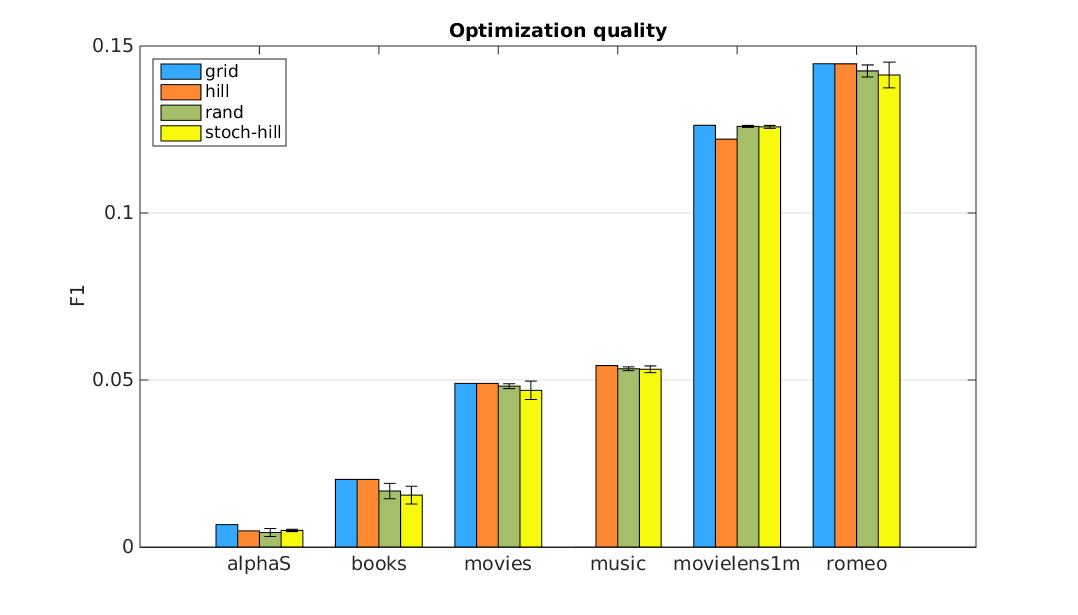
\includegraphics[width=0.9\textwidth]{fig/comp/comp_katz_quality.png}
    \caption{Comparison of the recommendation quality given from the parameters found by the different optimization strategies for \textit{katz-eig}.}
    \label{fig:comp_katz_quality}
\end{figure}

\FloatBarrier

\Figureref{fig:comp_katz_quality} show that all the evaluated strategies generate recommendations of a similar quality. The randomized algorithms \textbf{rand} and \textbf{stoch-hill} generally generate slightly worse recommendations due to the variance.

\begin{figure}[h!]
    \centering
    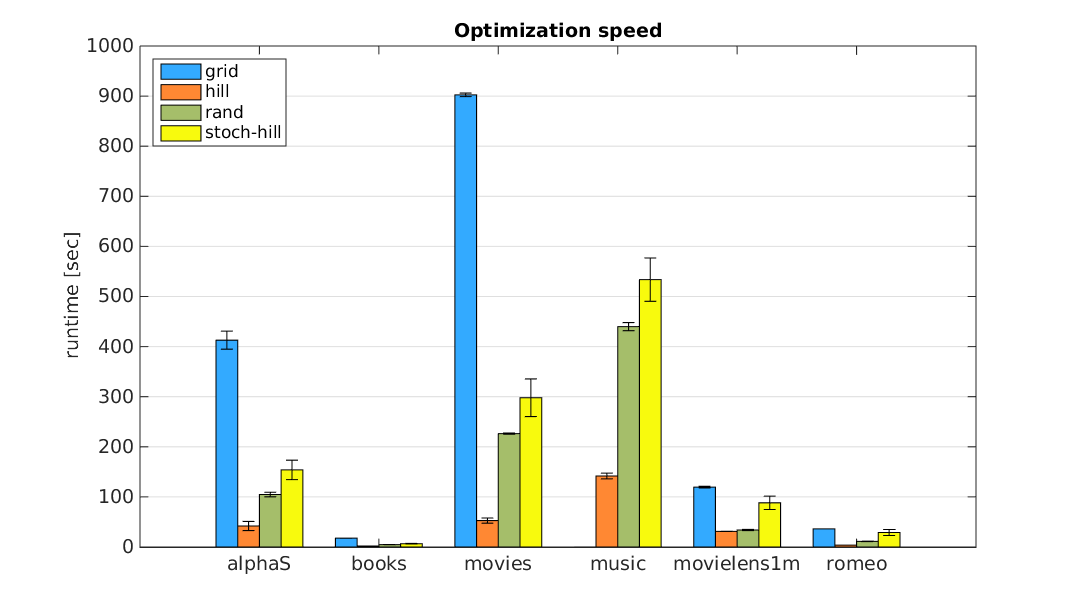
\includegraphics[width=0.9\textwidth]{fig/comp/comp_katz_speed.png}
    \caption{Comparison of the runtime of the different optimization strategies for \textit{katz-eig}, given the optimized parameters specified in \appendixref{app:opt_params}.}
\end{figure}

\begin{figure}[h!]
    \centering
    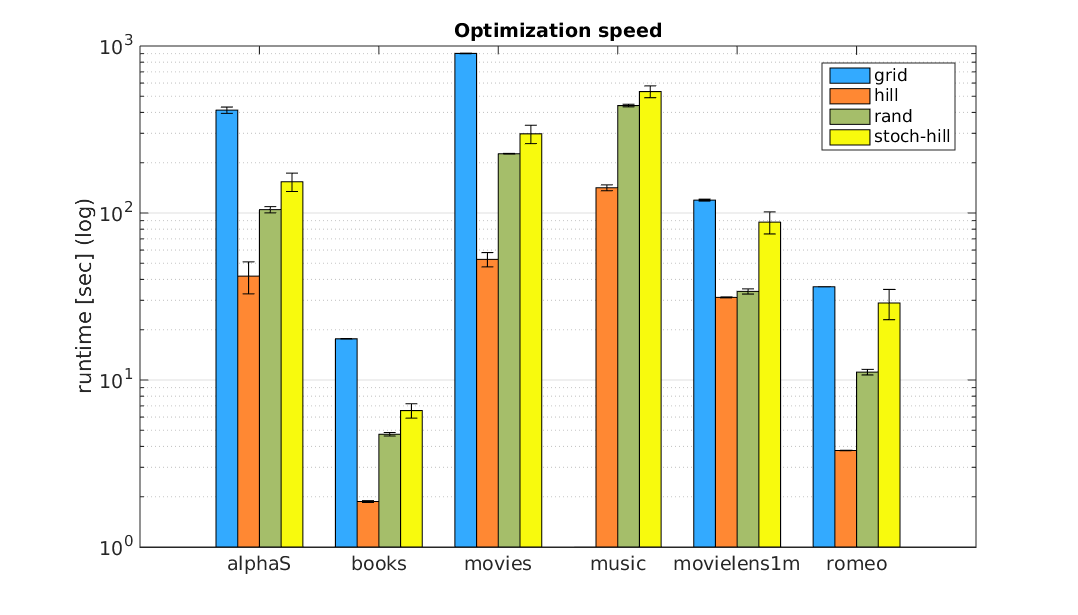
\includegraphics[width=0.9\textwidth]{fig/comp/comp_katz_speed_log.png}
    \caption{Comparison of the runtime of the different optimization strategies for \textit{katz-eig}, given the optimized parameters specified in \appendixref{app:opt_params}. In a log scale.}
\end{figure}

The runtime is very poor for the grid based approach as expected. The random algorithms also have poor performance, but this could be corrected by reducing the maximum number of samples they try. Reducing them might reduce the recommendation quality which already is worse than that of the regular hill climbing algorithm.

These tests show that the regular hill climbing algorithm is the best optimization strategy for \textit{katz-eig} producing similar recommendation quality to the full grid search while being much faster than the other alternatives.

